% 0359(본책 67쪽) — ∠A=90° 인 직각삼각형 ABC 의 내접원 O(접점 D, E, F · 원 색칠), BE=4 cm, CE=6 cm. 답(넓이)은 적지 않는다. 스캔 삽화를 TikZ 로 다시 그림.
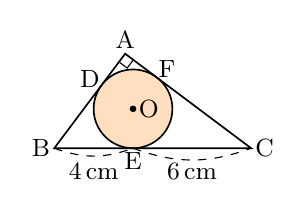
\begin{tikzpicture}[line width=0.6pt]
  \fill[orange!25] (1.000,0.500) circle (0.500);
  \draw (0.900,1.200) -- (0.000,0.000) -- (2.500,0.000) -- cycle;
  \draw (1.000,0.500) circle (0.500);
  \fill (1.000,0.500) circle (1.2pt);
  \draw[line width=0.4pt] (0.822,1.096) -- (0.926,1.018) -- (1.004,1.122);
  \draw[dashed, line width=0.4pt] (0.000,0.000) to[bend right=20] (1.000,0.000);
  \node[font=\small, inner sep=1.5pt] at (0.500,-0.300) {$4\,\mathrm{cm}$};
  \draw[dashed, line width=0.4pt] (1.000,0.000) to[bend right=20] (2.500,0.000);
  \node[font=\small, inner sep=1.5pt] at (1.750,-0.300) {$6\,\mathrm{cm}$};
  \node[font=\small, inner sep=1.5pt] at (0.900,1.370) {A};
  \node[font=\small, inner sep=1.5pt] at (-0.170,0.000) {B};
  \node[font=\small, inner sep=1.5pt] at (2.670,0.000) {C};
  \node[font=\small, inner sep=1.5pt] at (0.453,0.885) {D};
  \node[font=\small, inner sep=1.5pt] at (1.000,-0.160) {E};
  \node[font=\small, inner sep=1.5pt] at (1.430,1.009) {F};
  \node[font=\small, inner sep=1.5pt] at (1.200,0.500) {O};
\end{tikzpicture}
